\section{Ergebnisse}

In diesem Abschnitt werden die Ergbenisse diskutiert, welche sich aus der Berechnung des Kohlebedarfs und der Bestimmung der Zuerzeugungszeitpunkte ergeben haben. \autoref{fig:results-departures}a zeigt den berechneten Kohlebedarf für das Kraftwerk \emph{Jänschwalde} in Tonnen zwischen dem 25.01.2023 und dem 30.01.2023. Jeder Datenpunkt steht dabei für einen Zeitraum von 15 Minuten. Grau hinterlegt sind die Zeiträume A und B, welche in den Teilabbildungen \ref{fig:results-departures}b und \ref{fig:results-departures}c genauer betrachtet werden. \autoref{fig:results-departures}b zeigt den Zeitraum A vom 26.01. 12:00 bis 27.01. 12:00. Der Kohlebedarf ist in dieser Zeit praktisch konstant bei rund 750 t pro 15 Minuten. Die vertikalen roten Linien zeigen an, zu welchen Zeitpunkten ein Kohlezug erzeugt werden würde. Es ist zu beobachten, dass die Abstände dieser Linien zueinander verhältnismäßig gleichmäßig sind. \autoref{fig:results-departures}c zeigt den Zeitraum B vom 28.01. 12:00 bis 29.01. 12:00. In diesem Zeitraum unterliegt der Kohlebedarf einer deutlichen Schwankung. Der Zeitraum B ist zur weiteren Betrachtung in die Teilzeiträume B1 und B2 aufgeteilt, deren Grenze bei 00:00 Uhr (markiert durch die schwarze Strich-Punkt-Linie) liegt. Innerhalb von B1 liegt der Kohlebedarf bei etwa 700 t pro 15 Minuten. In B2 sinkt er auf ca. 400 bis 500 t pro 15 Minuten ab. Es ist zu erkennen, dass die Anzahl der in einer Zeitspanne erzeugten Kohlezüge direkt mit dem Kohlebedarf korreliert. Je höher also der Wert des Kohlebedarfs ist, desto mehr Züge werden erzeugt.

\begin{figure}[!ht]
	\centering
	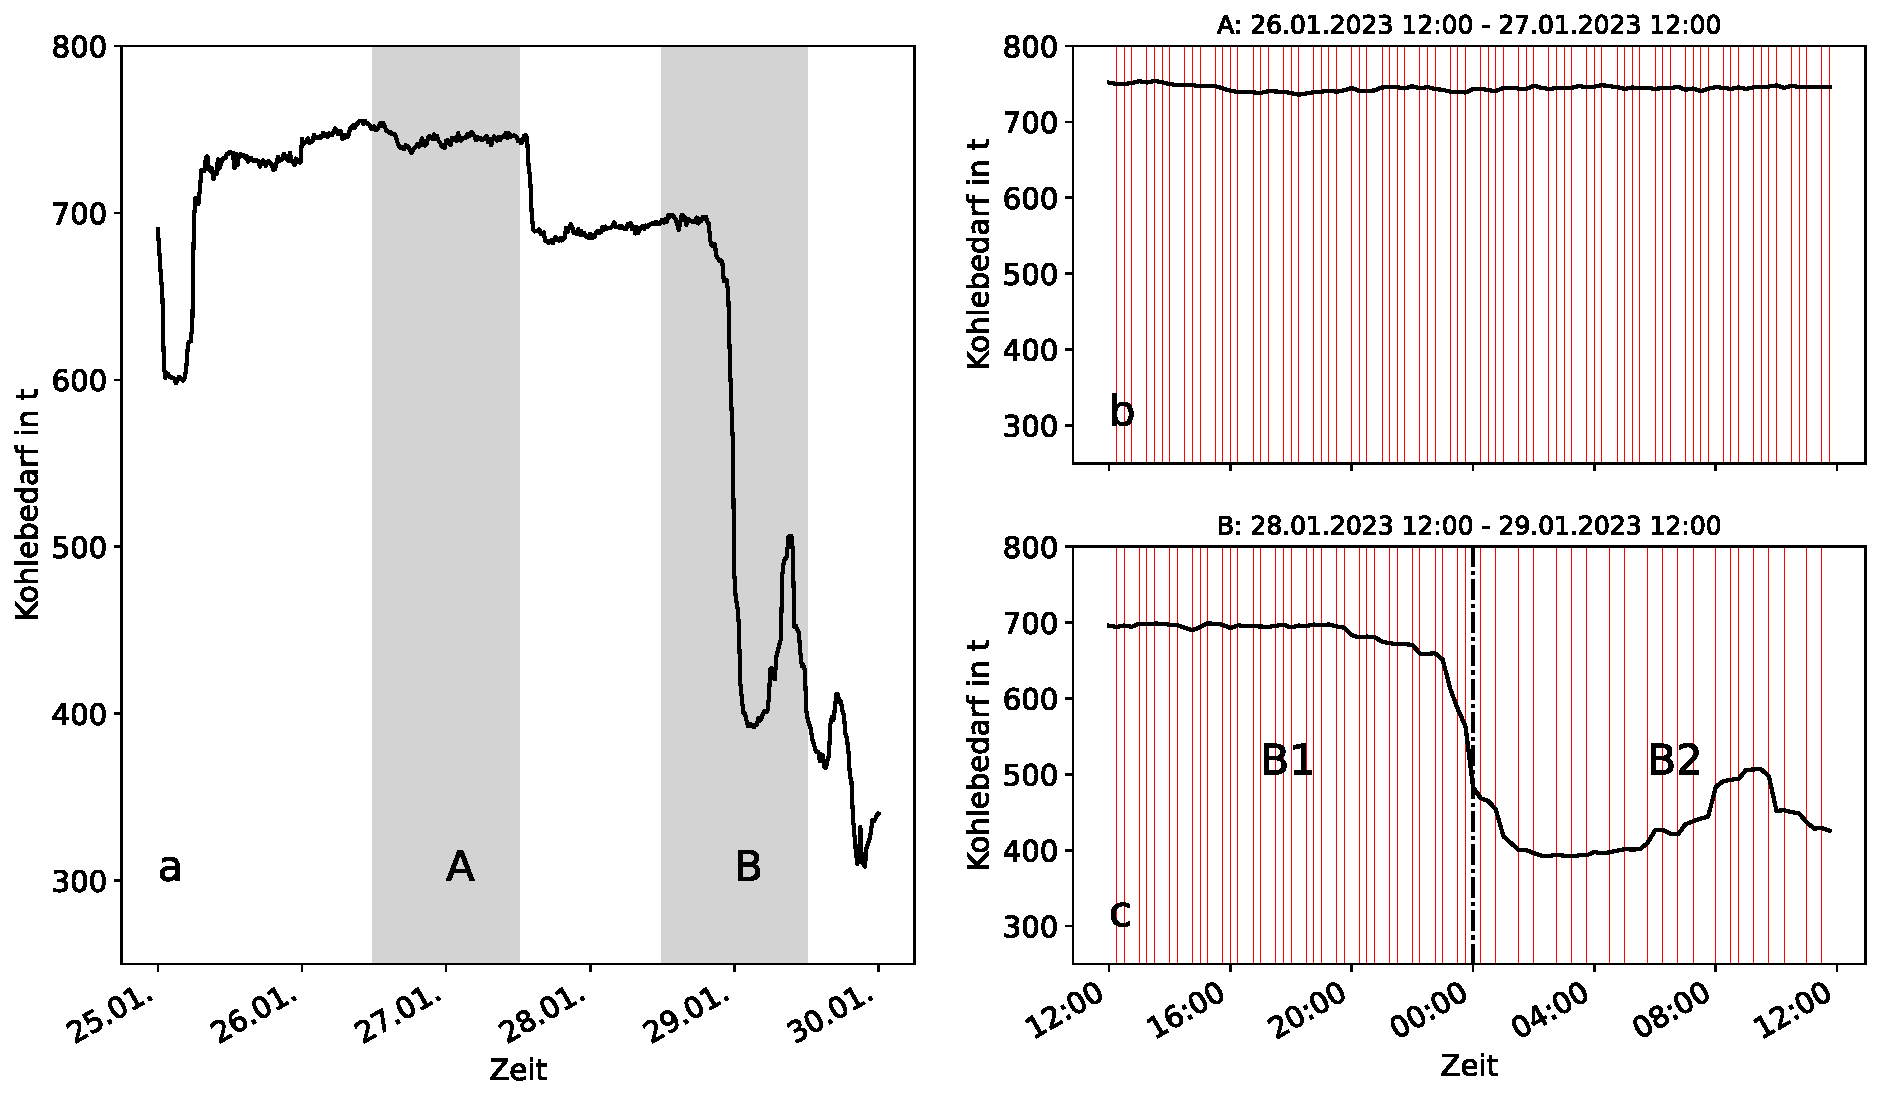
\includegraphics[width=1.0\linewidth]{images/results/departures.pdf}
	\caption{Kohlebedarf in Tonnen für das Kraftwerk \emph{Jänschwalde} zwischen dem 25.01.2023 und dem 30.01.2023 (a). Die Teilabbildungen b und c zeigen die Zeiträume A und B genauer. Die vertikalen, roten Punkt-Linien stellen die Abfahrtzeitpunkte von Kohlezügen dar. Die Strich-Punkt-Linie in Teilabbildung c teilt den Zeitraum in die Teilzeiträume B1 und B2 auf.}
	\label{fig:results-departures}
\end{figure}

\autoref{fig:results-periods} stellt die Daten aus \autoref{tab:results} grafisch dar. In \autoref{fig:results-periods}a sind die mittleren Abfahrtsperioden von Kohlezügen in Richtung Kraftwerk \emph{Jänschwalde} in den Zeiträumen A, B1 und B2 dargestellt. Es fällt auf, dass die Zeiträume A und B1 eine ähnliche Periodenlänge zwischen um 20 Minuten besitzen und die Periodenlänge in B2 mit etwa 34 Minuten deutlich höher ist.\\
\\
In \autoref{fig:results-periods}b sind die mittleren Abfahrtsperioden in Zeitraum A für die Kraftwerke \emph{Jänschwalde}, \emph{Boxberg} und \emph{Schwarze Pumpe} zu erkennen. Das Kraftwerk \emph{Jänschwalde} besitzt hierbei den niedrigsten Wert mit etwa 19 Minuten. Das Kraftwerk \emph{Boxberg} besitzt eine mittlere Abfahrtsperiode von ca. 28 Minuten und den höchsten Wert weist das Kraftwerk \emph{Schwarze Pumpe} mit rund 43 Minuten auf.

\begin{figure}[!ht]
	\centering
	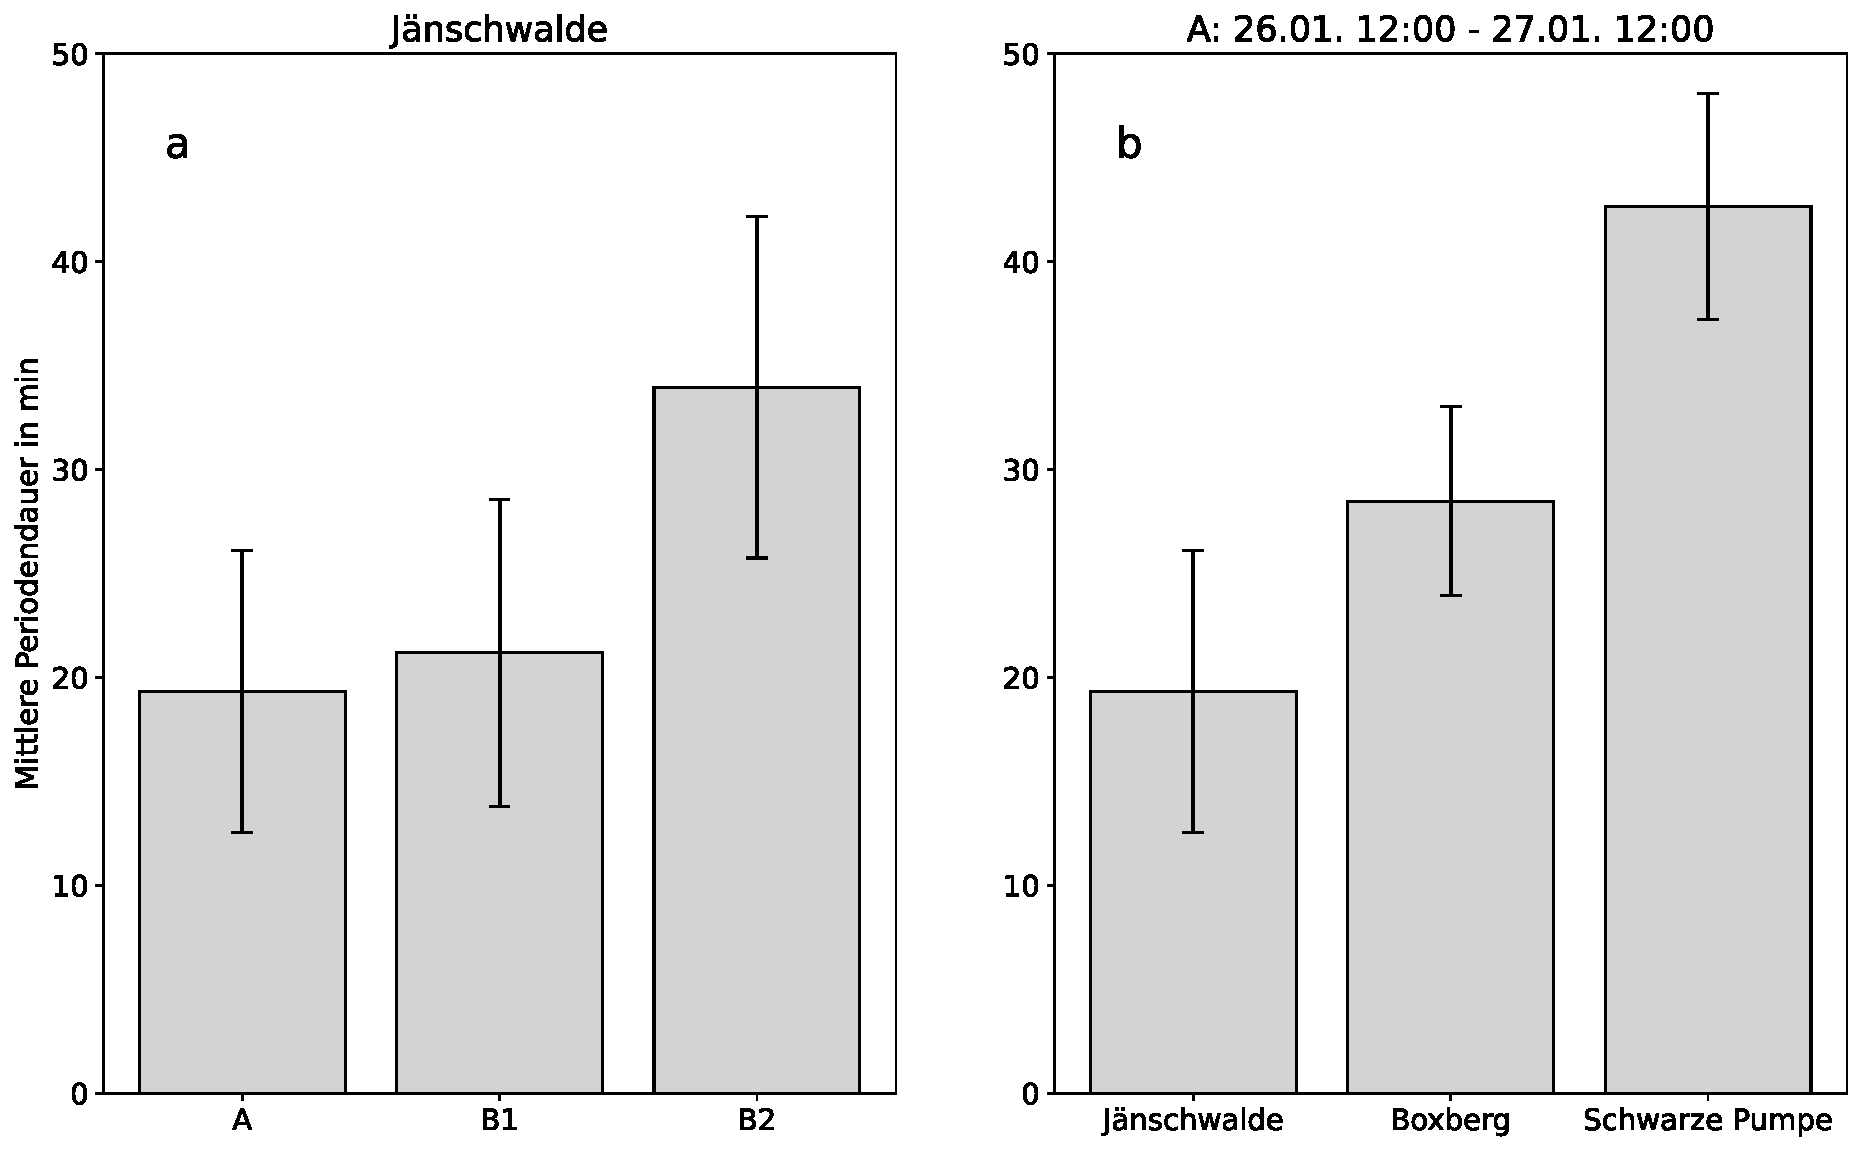
\includegraphics[width=1.0\linewidth]{images/results/periods.pdf}
	\caption{Mittlere Abfahrtsperioden in min für die drei Zeiträume A, B1 und B2 zum Karftwerk \emph{Jänschwalde} (a) und für die drei Kraftwerke \emph{Jänschwalde}, \emph{Boxberg} und \emph{Schwarze Pumpe} im Zeitraum A (b). Zeitraum A: 26.01. 12:00 - 27.01. 12:00, Zeitraum B1: 28.01. 12:00 - 29.01. 00:00, Zeitraum B2: 29.01. 00:00 - 29.01. 12:00}
	\label{fig:results-periods}
\end{figure}


\begin{table}[!ht]
	\centering
	\caption{Mittlere Abfahrtsperioden in min für die drei Zeiträume A, B1 und B2 zum Karftwerk \emph{Jänschwalde} (oberer Tabellenteil) und für die drei Kraftwerke \emph{Jänschwalde}, \emph{Boxberg} und \emph{Schwarze Pumpe} im Zeitraum A (unterer Tabellenteil). Zeitraum A: 26.01. 12:00 - 27.01. 12:00, Zeitraum B1: 28.01. 12:00 - 29.01. 00:00, Zeitraum B2: 29.01. 00:00 - 29.01. 12:00}
	\label{tab:results}
	\begin{tabular}{|l|r|}
		\hline
		\textbf{Zeitraum} & \textbf{Mittlere Abfahrtsperiode in min} \\
		\hline
		\hline
		A & $19,32 \pm 6,79$\\
		\hline
		B1 & $21,18 \pm 7,38$\\
		\hline
        B2 & $33,95 \pm 8,20$\\
		\hline
		\hline
        \textbf{Kraftwerk} & \\
		\hline
		\hline
        \emph{Jänschwalde} & $19,32 \pm 6,79$\\
		\hline
        \emph{Boxberg} & $28,47 \pm 4,54$\\
		\hline
		\emph{Schwarze Pumpe} & $42,66 \pm 5,45$\\
		\hline
	\end{tabular}
\end{table}